
\subsection*{1.}

\paragraph{a.} La fonction \( f_1 \) est dérivable sur \([0\,;\,10]\) en tant que composée de la fonction exponentielle et d'une fonction affine.

Pour tout réel \( x \) de l'intervalle \([0\,;\,10]\), on a : \( f_1'(t) = -0{,}57 \e^{-0{,}57t} \).

Ainsi \( f_1'(t) < 0 \) sur \([0\,;\,10]\).

La fonction \( f_1 \) est donc strictement décroissante sur \([0\,;\,10]\).

\paragraph{b.} Graphiquement, \( f_1(t) < 0{,}1 \) si \( t \) appartient à l'intervalle \( ]4\,;\,10] \) (valeur approchée pour 4).

La proportion de médicament est inférieure à \(0{,}1\) à partir de 4 heures.

\subsection*{2.}

\paragraph{a.} La fonction \( f_2 \) est dérivable sur \([0\,;\,10]\) en tant que produit de fonctions dérivables sur cet intervalle.

Pour tout réel \( t \) de l'intervalle \([0\,;\,10]\), on a :
\begin{align*}
f_2'(t) &= 1{,}75 \e^{-t} + 1{,}75t \times (-\e^{-t}) \\
&= 1{,}75 (1 - t) \e^{-t}.
\end{align*}

\paragraph{b.} La fonction exponentielle est strictement positive sur \( \mathbb{R} \).

Le signe de \( f_2'(t) \) ne dépend donc que de celui de \( 1 - t \).

\[
1 - t = 0 \iff t = 1 \quad \text{et} \quad 1 - t > 0 \iff t < 1
\]

On obtient donc le tableau de variations suivant :

\begin{center}
\begin{tikzpicture}
\tkzTabInit[lgt=3.5, espcl=4]{$x$ / 1, {Signe de $f'_2(t)$} / 1, {$f_2(t)$} / 2}{${0}$, ${1}$, ${10}$}
\tkzTabLine{,+,0,-,}
\tkzTabVar{-/{$0$},+/{$1{,}75\e^{-1}$},-/{$17{,}5\e^{-10}$}}{/}
\end{tikzpicture}
\end{center}

\paragraph{c.} La proportion de médicament dans le sang est la plus élevée au bout d'une heure \((t = 1)\).

